\documentclass{ctexart}
\usepackage{graphicx}
\usepackage{subfigure}
\usepackage{hyperref}
\usepackage{subfigure}
\usepackage{geometry}
\geometry{left=1.5cm,right=2.5cm,top=2.5cm,bottom=2.5cm}
\CTEXsetup[format+={\flushleft}]{section}

\begin{document}
\CJKfamily{li}
\title{周报}
\author{刘精昌}
\maketitle

\fangsong
\section*{本周工作}
\begin{itemize}
  \item 阅读《A Complexity-Invariant Distance Measure for Time Series》,文章比较简单,阅读的比较粗略,主要思想就是通过在距离前面添加系数,解决了序列分类中,将简单形状序列分类到复杂序列的情况。
  \item 阅读《FastDTW : Toward Accurate Dynamic Time Warping in Linear Time and Space》,文章将DTW方法的时间复杂度、空间复杂度从$O\left( n^2 \right)$ 降到 O(n),文章的成果很具有价值。
  \item 通过人造数据集和\href{http://www.cs.ucr.edu/~eamonn/time_series_data/}{TSDMA}数据集的实验,探究DTW方法、Euclid方法分类的精度差异,以及warp window大小对DTW方法分类精度的影响。人造数据是在一定的间隔上添加随机噪声而产生的,有四类,每类有四个训练集,四个测试集。TSDMA数据集的类数目,测试集、训练集数目都有给出。分类均采用1NN方法,因为计算量特别大,所以实验是在实验室服务器上利用MATLAB的并行计算完成的。主要结果如下:
      \begin{enumerate}
        \item 对于人造数据,从0到2递加间隔,每种间隔下,实验均运行100次(噪声是随机的),最后得到DTW距离和Euclid距离下的平均精度。实验结果曲线如图\ref{fig:1}。
            \begin{figure}
              \centering
              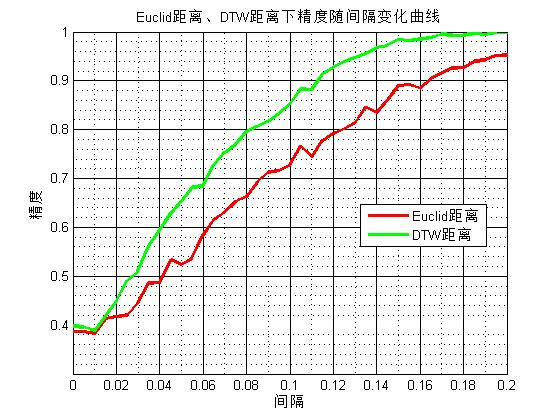
\includegraphics[width=0.6\textwidth]{1.jpg}
              \caption{Euclid、DTW距离下精度随时间变化}\label{fig:1}
            \end{figure}


            由实验结果曲线可以看出,DTW距离下的分类精度明显优于Euclid聚类。

        \item 对于不同的TSDMA数据集,分别应用DTW和Euclid距离,得到精度表

            \begin{flushleft}
              \begin{tabular}{|c|c|c|c|c|c|c|c|}
              \hline
              % after \\: \hline or \cline{col1-col2} \cline{col3-col4} ...
              name & Computers & Trace & FaceFour & WordsSynonyms & Gun\_Point & Plane & StrawBerry \\
              \hline
              lasses & 2 & 4 & 4 & 25 & 2 & 7 & 2 \\
              \hline
              training set size & 250 & 100 & 24 & 267 & 50 & 105 & 370 \\
              \hline
              test set size & 250 & 100 & 88 & 638 & 150 & 105 & 613 \\
              \hline
              sequence length & 720 & 275 & 350 & 270 & 150 & 144 & 235 \\
              \hline
              error rate (Euclid) & 0.424 & 0.24 & 0.21591 & 0.38245 & 0.086667 & 0.038095 & 0.06199 \\
              \hline
              error rate (DTW) & 0.332 & 0.01 & 0.15909 & 0.32445 & 0.12 & 0 & 0.66884 \\
              \hline
            \end{tabular}
            \end{flushleft}

            从上面的精度表看以看出,大部分情况下dtw距离的精度都要优于Euclid距离,个别的数据dtw距离的精度反而不如Euclid距离。
        \item 主要探究warp window的变化对DTW距离精度的影响。实验数据是间隔为0.135的人造数据和部分TSDMA数据,方法是将warp window从0到1每次变化1\% ,记录精度的变化,结果如图\ref{fig:side:a}、\ref{fig:side:b}、\ref{fig:side:c}、\ref{fig:side:d}、\ref{fig:2}所示。

            \begin{figure}
                \begin{minipage}{0.5\linewidth}
                \centering
                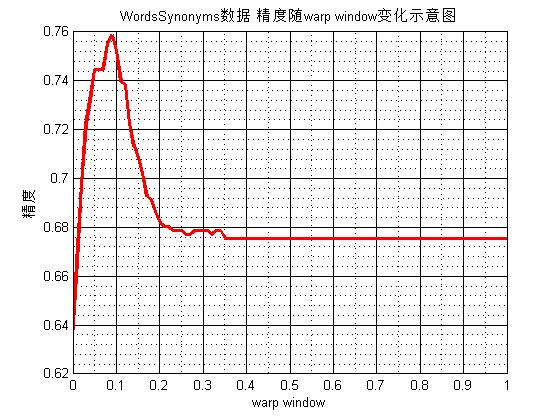
\includegraphics[width=3in]{6.jpg}
                \caption{WordsSunonyms数据集}
                \label{fig:side:a}
                \end{minipage}%
                \hfill
                \begin{minipage}{0.5\linewidth}
                \centering
                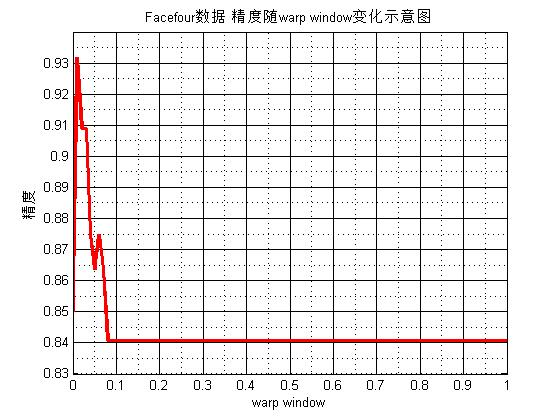
\includegraphics[width=3in]{3.jpg}
                \caption{FaceFoue数据集}
                \label{fig:side:b}
                \end{minipage}
                \vfill
                \begin{minipage}{0.5\linewidth}
                \centering
                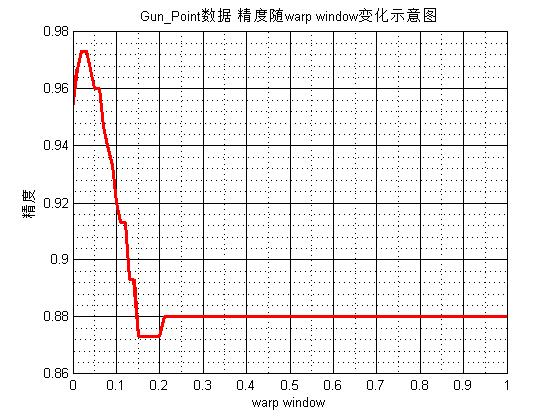
\includegraphics[width=3in]{4.jpg}
                \caption{Gun\_Point数据集}
                \label{fig:side:c}
                \end{minipage}
                \hfill
                \begin{minipage}{0.5\linewidth}
                \centering
                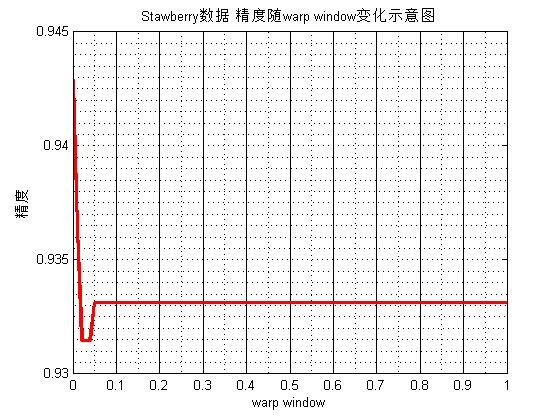
\includegraphics[width=3in]{5.jpg}
                \caption{StrawBerry数据集}
                \label{fig:side:d}
                \end{minipage}
            \end{figure}
            
            \begin{figure}
              \centering
              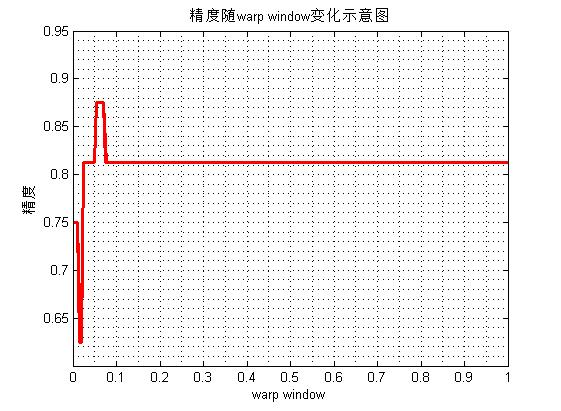
\includegraphics[width=0.6\textwidth]{2.jpg}
              \caption{人造数据集}\label{fig:2}
            \end{figure}
            
            从这些图中可以看出,一般而言,一个较小的warp window(小于10\%)对DTW分类精度的提升是有利的。
      
      \end{enumerate}
      

\end{itemize}

\section*{下周计划}
\begin{itemize}
  \item 主要写毕设论文,灵活地进行实验,参考论文。
\end{itemize}

\end{document} 